% $HeadURL$

\subsection{Glyph: \glyph{Unspecified entity}}
\label{sec:unspecifiedEntity}

The simplest type of EPN is the \glyph{unspecified entity}: one whose type is unknown or simply not relevant to the purposes of the map.
This arises, for example, when the existence of the entity has been inferred indirectly, or when the entity is merely a construct introduced for the needs of a map, without direct biological relevance.
These are examples of situations where the \emph{unspecified entity} glyph is appropriate.
(Conversely, for cases where the identity of the entities composing the pool is known, there exist other, more specific glyphs described elsewhere in the specification.)

\begin{glyphDescription}

\glyphSboTerm
 SBO:0000285 ! material entity of unspecified nature


\glyphIncoming
Zero or more \glyph{production} arcs (\sect{production}).



\glyphOutgoing
Zero or more \glyph{consumption} arcs (\sect{consumption}), \glyph{modulation arcs} (\sect{modulations}), \glyph{logic arcs} (\sect{logicArc}), or \glyph{equivalence arcs} (\sect{equivalenceArc}).


\glyphContainer
A \glyph{unspecified entity} is represented by an elliptic shape, as shown in \fig{unspecified}.
Note that the shape must remain an ellipse to avoid confusion with \glyph{simple chemical}, which is represented with a stadium shape (\sect{simpleChemical}).

\glyphLabel
A \glyph{unspecified entity} is identified by a label  that is a string of characters that may be distributed on several lines to improve readability.
The centre of the label must be placed on the centre of the container.
The label may extend outside of the container.



\glyphAux
An \glyph{unspecified entity} can carry a \glyph{clone marker} (see \sect{cloneMarker}).

\end{glyphDescription}

\begin{figure}[H]
  \centering
  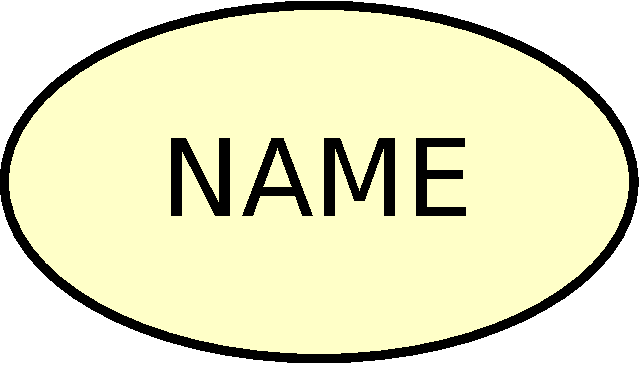
\includegraphics{images/unspecified}
  \caption{The \PD glyph for \glyph{unspecified entity}.}
  \label{fig:unspecified}
\end{figure}

% The following is for [X]Emacs users.   Please leave in place.
% Local Variables:
% TeX-master: "../sbgn_PD-level1"
% End:
